\documentclass[twocolumn,twoside,11pt,a4paper]{article}
%----------------------------------------------------------------------------------------
%	packages
%----------------------------------------------------------------------------------------

%\usepackage[portuguese]{babel}  % portuguese
\usepackage{graphicx}           % images: .png or .pdf w/ pdflatex; .eps w/ latex
\usepackage{lipsum}             % generate dummy text throughout this template

%% For iso-8859-1 (latin1), comment next line and uncomment the second line
\usepackage[utf8]{inputenc}
%\usepackage[latin1]{inputenc}

\usepackage[T1]{fontenc}        % T1 fonts
\usepackage{lmodern}            % fonts
\usepackage[sc]{mathpazo}       % Use the Palatino font
\linespread{1.00}               % Line spacing - Palatino needs more space between lines
\usepackage{microtype}          % Slightly tweak font spacing for aesthetics
\usepackage{url}                % urls
\usepackage[hang, small, labelfont=bf,up,textfont=it,up]{caption} % Custom captions under/above floats in tables or figures
\usepackage{booktabs}           % Horizontal rules in tables
\usepackage{float}              % Required for tables and figures in the multi-column environment - they need to be placed in specific locations with the [H] (e.g. \begin{table}[H])
\usepackage{paralist}           % Used for the compactitem environment which makes bullet points with less space between them

% geometry package
\usepackage[outer=19mm,inner=19mm,vmargin=13mm,includehead,includefoot,headheight=15pt]{geometry}
%% space between columns
\columnsep 10mm

\usepackage{abstract}           % Allows abstract customization
\renewcommand{\abstractnamefont}{\normalfont\bfseries} % Set the "Abstract" text to bold
\renewcommand{\abstracttextfont}{\normalfont\small\itshape} % Set the abstract itself to small italic text

% \usepackage{titlesec}           % Allows customization of titles
% \renewcommand\thesection{\Roman{section}} % Roman numerals for the sections
% \renewcommand\thesubsection{\Roman{subsection}} % Roman numerals for subsections
% \titleformat{\section}[block]{\large\scshape\centering}{\thesection.}{1em}{} % Change the look of the section titles
% \titleformat{\subsection}[block]{\large}{\thesubsection.}{1em}{} % Change the look of the section titles

\usepackage[pdftex]{hyperref}
\hypersetup{%
    a4paper = true,              % use A4 paper 
    bookmarks = true,            % make bookmarks 
    colorlinks = true,           % false: boxed links; true: colored links
    pdffitwindow = false,        % page fit to window when opened
    pdfpagemode = UseNone,       % do not show bookmarks
    pdfpagelayout = SinglePage,  % displays a single page
    pdfpagetransition = Replace, % page transition
    linkcolor=blue,              % hyperlink colors
    urlcolor=blue,
    citecolor=blue,
    anchorcolor=green
}

\usepackage{indentfirst}         % indent also 1st paragraph

\usepackage{fancyhdr}            % Headers and footers
\pagestyle{fancy}                % pages have headers and footers
\fancyhead{}                     % Blank out the default header
\fancyfoot{}                     % Blank out the default footer
\fancyhead[LO,RE]{Wordify: Bridging Multilingual Knowledge Bases for Seamless Entity Disambiguation} % Custom header text
\fancyhead[RO,LE]{\thepage}      % Custom header text
\fancyfoot[RO,LE]{Group D, \today} % Custom footer text
\renewcommand{\headrulewidth}{0.4pt}
\renewcommand{\footrulewidth}{0.4pt}

%\hyphenation{}                  % explicit hyphenation

%----------------------------------------------------------------------------------------
%	macro definitions
%----------------------------------------------------------------------------------------

% entities
\newcommand{\class}[1]{{\normalfont\slshape #1\/}}
\newcommand{\svg}{\class{SVG}}
\newcommand{\scada}{\class{SCADA}}
\newcommand{\scadadms}{\class{SCADA/DMS}}

% utils commands

\newcommand\todo[1]{\textcolor{red}{\{#1\}}}

%----------------------------------------------------------------------------------------
%	TITLE SECTION
%----------------------------------------------------------------------------------------

\title{\vspace{-15mm}\fontsize{24pt}{10pt}\selectfont\textbf{Wordify: Bridging Multilingual Knowledge Bases for Seamless Entity Disambiguation}} % Article title

\author{Fábio Araújo de Sá\\
\small \texttt{up202007658@up.pt}\\
\and
Marcos Rafael Peixoto Aires\\
\small \texttt{up202006888@up.pt}
\and
Pedro Pereira Ferreira\\
\small \texttt{up202004986@up.pt}
\vspace{-5mm}
}

\date{\today}

%----------------------------------------------------------------------------------------

\begin{document}

\maketitle
\thispagestyle{plain}

%----------------------------------------------------------------------------------------
%	ABSTRACT
%----------------------------------------------------------------------------------------

\begin{abstract}

Wordify is a multilingual entity disambiguation system leveraging Web Semantics and Linked Data principles to address challenges in identifying and linking entities across diverse knowledge bases. By using technologies such as RDF, SPARQL, SKOS, and OWL, Wordify bridges data from sources like DBpedia and Wikidata to resolve ambiguities and detect false friends. Its user-friendly interface simplifies entity searches, supports language-specific filtering, and adheres to Tim Berners-Lee's principles for structured, interconnected data. This paper discusses Wordify’s architecture, key functionalities, and limitations, highlighting its potential to improve cross-lingual knowledge base interoperability.

\end{abstract}

%----------------------------------------------------------------------------------------
%	ARTICLE CONTENTS
%----------------------------------------------------------------------------------------

\section{Introduction}\label{sec:intro}

In Web Semantics and Linked Data contexts, it is common to handle a significant number of entities derived from the Web. Moreover, those are stored in various Knowledge Bases (KBs), such as the WikiData \cite{wikidata} and DBPedia \cite{dbpedia}, containing various entities, which majority of them are related to each other. In the worst cases, the entities are associated with the equivalent ones in several languages.

However, it's difficult to link these types of data. In fact, there's no simple way to connect similar information across KBs because the way the information is organized in the KBs varies. Also, an entity may have multiple entries because it has multiple values in the same or different knowledge bases, which makes it unclear what the entity is.

To overcome the aforementioned challenges, it would be ideal to build a system capable to link these entities across the different KBs, so that a computer could disambiguate them. As a result, it was built Wordify. Wordify is a system that disambiguates existing entities, possibly in different languages, using Web Semantics and Linked Data principles \cite{kn:tbl}, concepts, and technologies. It will help a computer and humans to perceive which entity is being referred to, if it is ambiguous in a certain context, or to consult false friends between languages.

This paper presents a proposal for a Wordify application to address the ambiguity problem. It covers the motivation, requirements, and state-of-the-art solutions. The application architecture is detailed in Section~\ref{sec:application}, highlighting the interconnectedness of frameworks and tools. Section~\ref{sec:discussion} discusses the results of the proposed solution, as well as challenges and limitations. The paper concludes in Section~\ref{sec:conclusions} with the future work, accompanied by references and annexes.

%------------------------------------------------

\section{Motivation}\label{sec:motivation}

Humans always tried to communicate in a clear and simple way with others, as well as with computers. However, it is a critical, inherent problem of the languages used by humans to communicate, as they are ambiguous. As a result, the entities present in the Web are also equivocal in some cases.

It is easy to think of a word, or something that can have different meanings, for different contexts: for instance, when someone is talking about a ``balance'', this word can mean the state in which opposing forces, or can also mean the object used to measure weights.

Another problem faced with natural languages is the fact that the same word can also have divergent meanings in different languages (false friends): the word ``citrine'' in some contexts, can refer to a yellow gemstone or a yellowish color. Similarly, the word ``tuna'' in English refers to a group of fishes, while in Portuguese, it refers to a musical academic group. As a consequence, it becomes difficult to connect the same word to distinct entities, especially when used in different domains.

With the exposure of this problem, it is clear there is the necessity for a system that can manipulate a knowledge base in a manner that elucidates the entities' search, regarding the multi-language characteristics and contexts. To this end, the Wordify system was developed.

\section{Functionalities \& Requirements}\label{sec:requirements}

In light of the emphasis placed on comprehending the significance of our system and the rationale behind the relevance of our solution in the preceding section, the following one will describe the key functionalities of our solution. 

Firstly, the basic capability of our system is to link various entities to the input search term. Thus, by means of example, if a user searches for ``tuna'', our prototype links this word with the entities that are associated with it. Moreover, various definitions, as well as their respective languages, are linked to the entities retrieved. If the word ``tuna'', is associated with two entities, each of those can be connected with one or more definitions, each of which is linked to a certain language. Figure \ref{fig:retrieval} provides a generic example of the aforementioned flow. 

Moreover, the system must be capable to filter the search results by a language selected by the user. If none is selected, it will be used english by default on the entity retrieving process. For instance, if the user wants to look for the entity ``chat'' in french, they must choose the ``French'' option, when they start their search using Wordify.

Furthermore, our system offers two other functionalities, namely entity disambiguation and detection of false friends. The former consists in showing the different meanings that a certain word can have in a specific language. The latter consist in words that are written in the same way in different languages (multilingual homographs) but have distinct meaning. For example, the word ``citrine'' has meaning both in italian and english. However, in italian it refers to a mineral, and in english to a shade of the color yellow.

In addition to these features, it is possible to see what are the most likely languages the entities may belong to. This functionality calculates the ratio between the number of times a language is associated to the retrieved entities, and the sum of languages for all the retrieved entities, when a search occurs.

Our system adheres to the Tim Berners-Lee’s four principles \cite{kn:tbl}, which serve as essential guidelines for publishing and interconnecting structured data on the web. These principles support the evolution of the Semantic Web, promoting the creation of a data web that is machine-readable, interoperable, and richly interconnected. 

The first one consists in using Uniform Resource Identifiers (URIs) to identify resources, as URIs are the foundation for identifying and referencing resources unambiguously on the web. The second principle lies in using HTTP URIs, allowing users and machines to retrieve data.
This makes resources discoverable, reusable, and linkable across datasets. The third one aims to provide useful information in standard formats according to the Resource Description Framework (RDF) \cite{rdf}, considering that the returned data should describe the resource and its relationships to other resources. Finally, the last highlighted principle by Tim Berners-Lee is centered on including links to other URIs to connect data, enabling navigation and discovery across datasets, as these links create a connected web of data, similar to how hyperlinks connect web pages.

\section{Existing Approaches}\label{sec:sota}

This section details three related existing works that also aim to address entity disambiguation on the Web.

\begin{itemize}

    \item \textbf{DBPedia Spotlight \cite{kn:DBS}}: is an entity disambiguation tool that uses DBpedia to identify and link entities in texts. It applies Natural Language Processing (NLP) techniques to connect terms to URIs.

    \item \textbf{Wikidata Query Service \cite{kn:WQS}}: provides an interface for SPARQL \cite{sparql} queries, allowing the retrieval of structured data about entities in Wikidata, facilitating data integration and disambiguation across different resources and languages. Besides the SPARQL interface, it also permits the user to visualize queries as tables, maps, graphs, and timelines, making the data more comprehensible.

    \item \textbf{YAGO \cite{kn:YAGO}}: semantic knowledge base that organizes knowledge in an RDF ontology and provides links to various sources, such as DBpedia, Wikidata and WordNet \cite{wordnet}. It is used for entity disambiguation and building semantic relationships across multiple contexts. These semantic relationships can be hierarchical (e.g., ``is-a'') and non-hierarchical (e.g., ``located-in'', ``works-at'').
    
\end{itemize}

Those works can, in fact, show to the user in a simple and clear way what one or more entities can refer to. However, their users need to know how those entities are represented, as well as a solid background of the languages used in this context, especially SPARQL and RDF. As a result,ordify provides a more user-friendly interface, allowing users to search for those entities, without needing to know how they are organized, neither using a structured code to make that query.

%------------------------------------------------

\section{Architecture}\label{sec:application}

The proposed architecture for Wordify's development is illustrated in Figure \ref{fig:architecture}. To meet the system requirements, the application leverages a Docker \cite{docker} deployment for portability, a web interface to facilitate end-user interaction with data, and SPARQL for querying resources in DBpedia and Wikidata. It employs Simple Knowledge Organization System (SKOS) \cite{skos} to organize concepts, catalog synonyms, and manage hierarchies for ambiguous terms, enabling seamless integration of different data sources. Additionally, Web Ontology Language (OWL) \cite{owl} is used to differentiate word interpretations, resolve ambiguities, and identify false friends across entities.

\subsection{RDF Graph Structure}

Given a user-provided word in a specific language, the system performs SPARQL queries on the selected knowledge databases to retrieve the possible entities associated with the input and, for each entity, its meaning in the available languages. The results, returned in RDF format, are then used to construct a graph, also in RDF, which supports more structured queries aligned with Wordify's needs and requirements. The structure of the resulting graph is outlined in Figure \ref{fig:graph}.

The graph has its root at the user's input, cataloged using ``SKOS.Concept'' as the primary concept. Then, for each entity identified, it associates the entity to the user input using the predicate ``SKOS.Related''. Subsequently, for each of these entities, it links all the definitions found, and for each definition, the associated language. The predicates ``SKOS.Lang'' and ``SKOS.Definition'' are employed for these associations. Finally, the knowledge database consulted to locate the entity is linked using the predicate ``OWL.Source''. Where applicable, the predicates ``OWL.FalseFriend'' and ``OWL.Ambiguity'' are also applied between entities. Thus, both SKOS and OWL were used to meaningfully link different elements from various sources. The data transformation process for inclusion in this graph follows a proposal aimed at minimizing duplicate data as much as possible.

\subsection{Computing Ambiguities}

From the graph created and detailed in the previous subsection, it is easy to obtain pairs of entities for the same input where ambiguities occur. An ambiguity arises between two entities, as shown in Figure \ref{fig:graph-ambiguities}, when there is a language in the system that returns different meanings for the same input.

\subsection{Computing False Friends}

Given the nature and structure of Wordify's internal graph, searching for pairs of entities that are false friends is also straightforward. False friends occur when entities with different connotations are found between two different languages. An example is present in Figure \ref{fig:graph-ff}.

\subsection{Computing Top Languages}

The presentation of the top five languages in percentage in Wordify is ensured through a simple query to the leaves/languages, considering all the entities in the system resulting from the user's input, followed by mathematical computation, as shown in Figure \ref{fig:graph-languages}. This feature enables the system to infer, based solely on the data returned by the knowledge sources, the language in which the input might have been written. In other words, given a text containing the user's input word, the system can compute the probable language of that text.

%------------------------------------------------

\section{Discussion}\label{sec:discussion}

With the Wordify architecture, the Tim Berner-Lee's Four Principles \cite{kn:tbl} are satisfied successfully. In fact, it is possible to perceive the accomplishment of the first two: all the entities are identified with a unique URI. Moreover, it provides useful information in standard formats, as the entities are all structured in RDF. Furthermore, the user can use HTTP URIs to look up for data, since each entity has a URI associated to it (/search/<entity\-name>/), as well as they can access to other URIs present in each entities' page, to see the respective ambiguities and false friends.

There are some limitations that were considered before the inception of Wordify. Firstly, the vast number of potential entities that could be ambiguous, both within and across different languages, poses a computational challenge. To mitigate this and reduce processing time, we limited the number of entities retrieved.

Moreover, there are instances where a word may exist in one language but cannot be automatically associated with another representation in another entity in a different language. For instance, "saudade" means missing someone in portuguese, but there is no direct english translation. Unfortunately, there is no direct solution to overcome this challenge with the current Wordify's implementation.

Although our system is able to disambiguate entities and present false friends, it faces some limitations, which we consider in this section as well.

The first one is related to the difficulty of finding definitions in specific languages. The search feature of our prototype supports only seven languages, limiting the range of available language options to search in. This limitation can be observed in Figure \ref{fig:limitedLanguages}.

The second limitation pertains to the integration of data from the two knowledge sources utilized, DBpedia and Wikidata. When a user searches for the same entity and applies a source filter, the entity retrieved from Wikidata differs from the one retrieved from DBpedia. This discrepancy is evident in their distinct meanings, top five languages, and ambiguities, as illustrated in Figure \ref{fig:crossDataLimitation}.

The third limitation of our system relates to the inability to identify regionalisms due to the absence of detailed geographical data for the countries whose languages are being searched. For instance, as illustrated in Figure \ref{fig:imperialVSFine}, our system cannot distinguish between ``fino'' and ``imperial'', two Portuguese terms specific to Porto and Lisbon, respectively. This limitation arises because the prototype lacks geographical data about specific regions within countries.

Finally, users are also limited to search for single words in our system, as it is not tailored for searches with more than one word, as it can be seen in Figure \ref{fig:Beaks}.

%------------------------------------------------

\section{Conclusions}\label{sec:conclusions}

Wordify demonstrates the potential to enhance cross-lingual entity disambiguation and knowledge base interoperability. By leveraging Web Semantics and Linked Data principles, the system offers a user-friendly interface that simplifies complex operations such as linking entities across diverse knowledge bases and resolving ambiguities. Despite its success in adhering to standards such as RDF and OWL and providing functionality for detecting false friends, Wordify is limited by its support for a small subset of languages, difficulties in addressing regionalisms, and the inability to process multi-word queries.

Future improvements could focus on expanding language support, incorporating detailed geographical metadata to better handle regionalisms, and enabling multi-word input processing. Addressing these limitations will further enhance Wordify's role as a tool in bridging multilingual knowledge bases, fostering better understanding, and enabling seamless integration of the data of Web.

%----------------------------------------------------------------------------------------
%	REFERENCES
%----------------------------------------------------------------------------------------

\bibliographystyle{unsrt-pt}
\bibliography{artigo}

%--------------------------------------------------------------------------------------
%	Annexes
%----------------------------------------------------------------------------------------

\section{Annexes} \label{sec:annexes}

\textit{On the following page.}

\begin{figure*}
  \begin{center}
    \leavevmode
    \includegraphics[width=0.64\textwidth]{Images/entityStructure.png}
    \caption{Example of a retrieved entity's structured.}
    \label{fig:retrieval}
  \end{center}
\end{figure*}

\begin{figure*}
  \begin{center}
    \leavevmode
    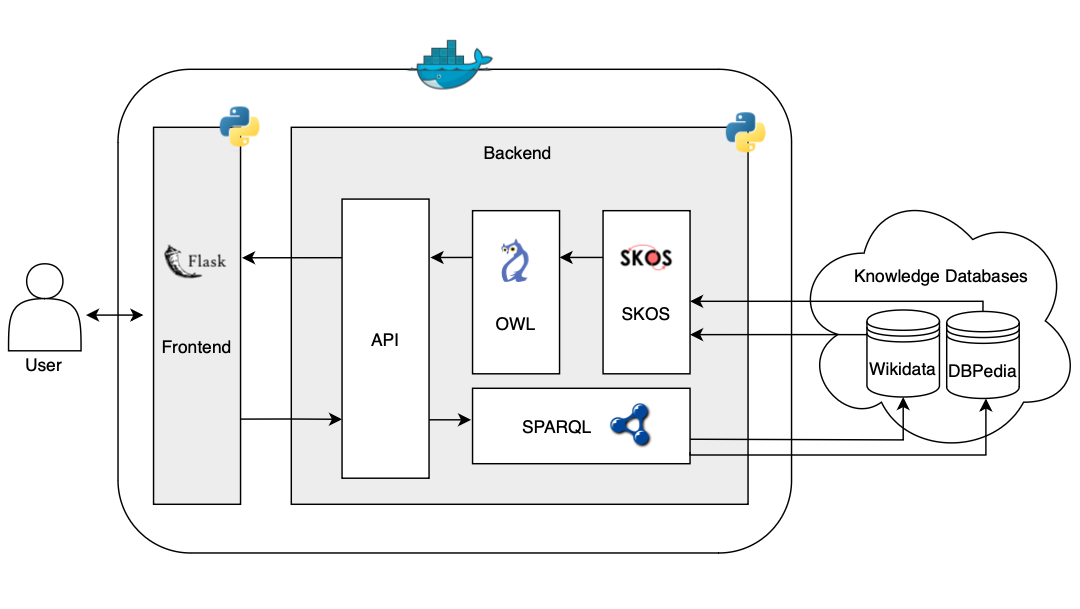
\includegraphics[width=0.65\textwidth]{Images/architecture.png}
    \caption{Wordify's architecture}
    \label{fig:architecture}
  \end{center}
\end{figure*}

\begin{figure*}
  \begin{center}
    \leavevmode
    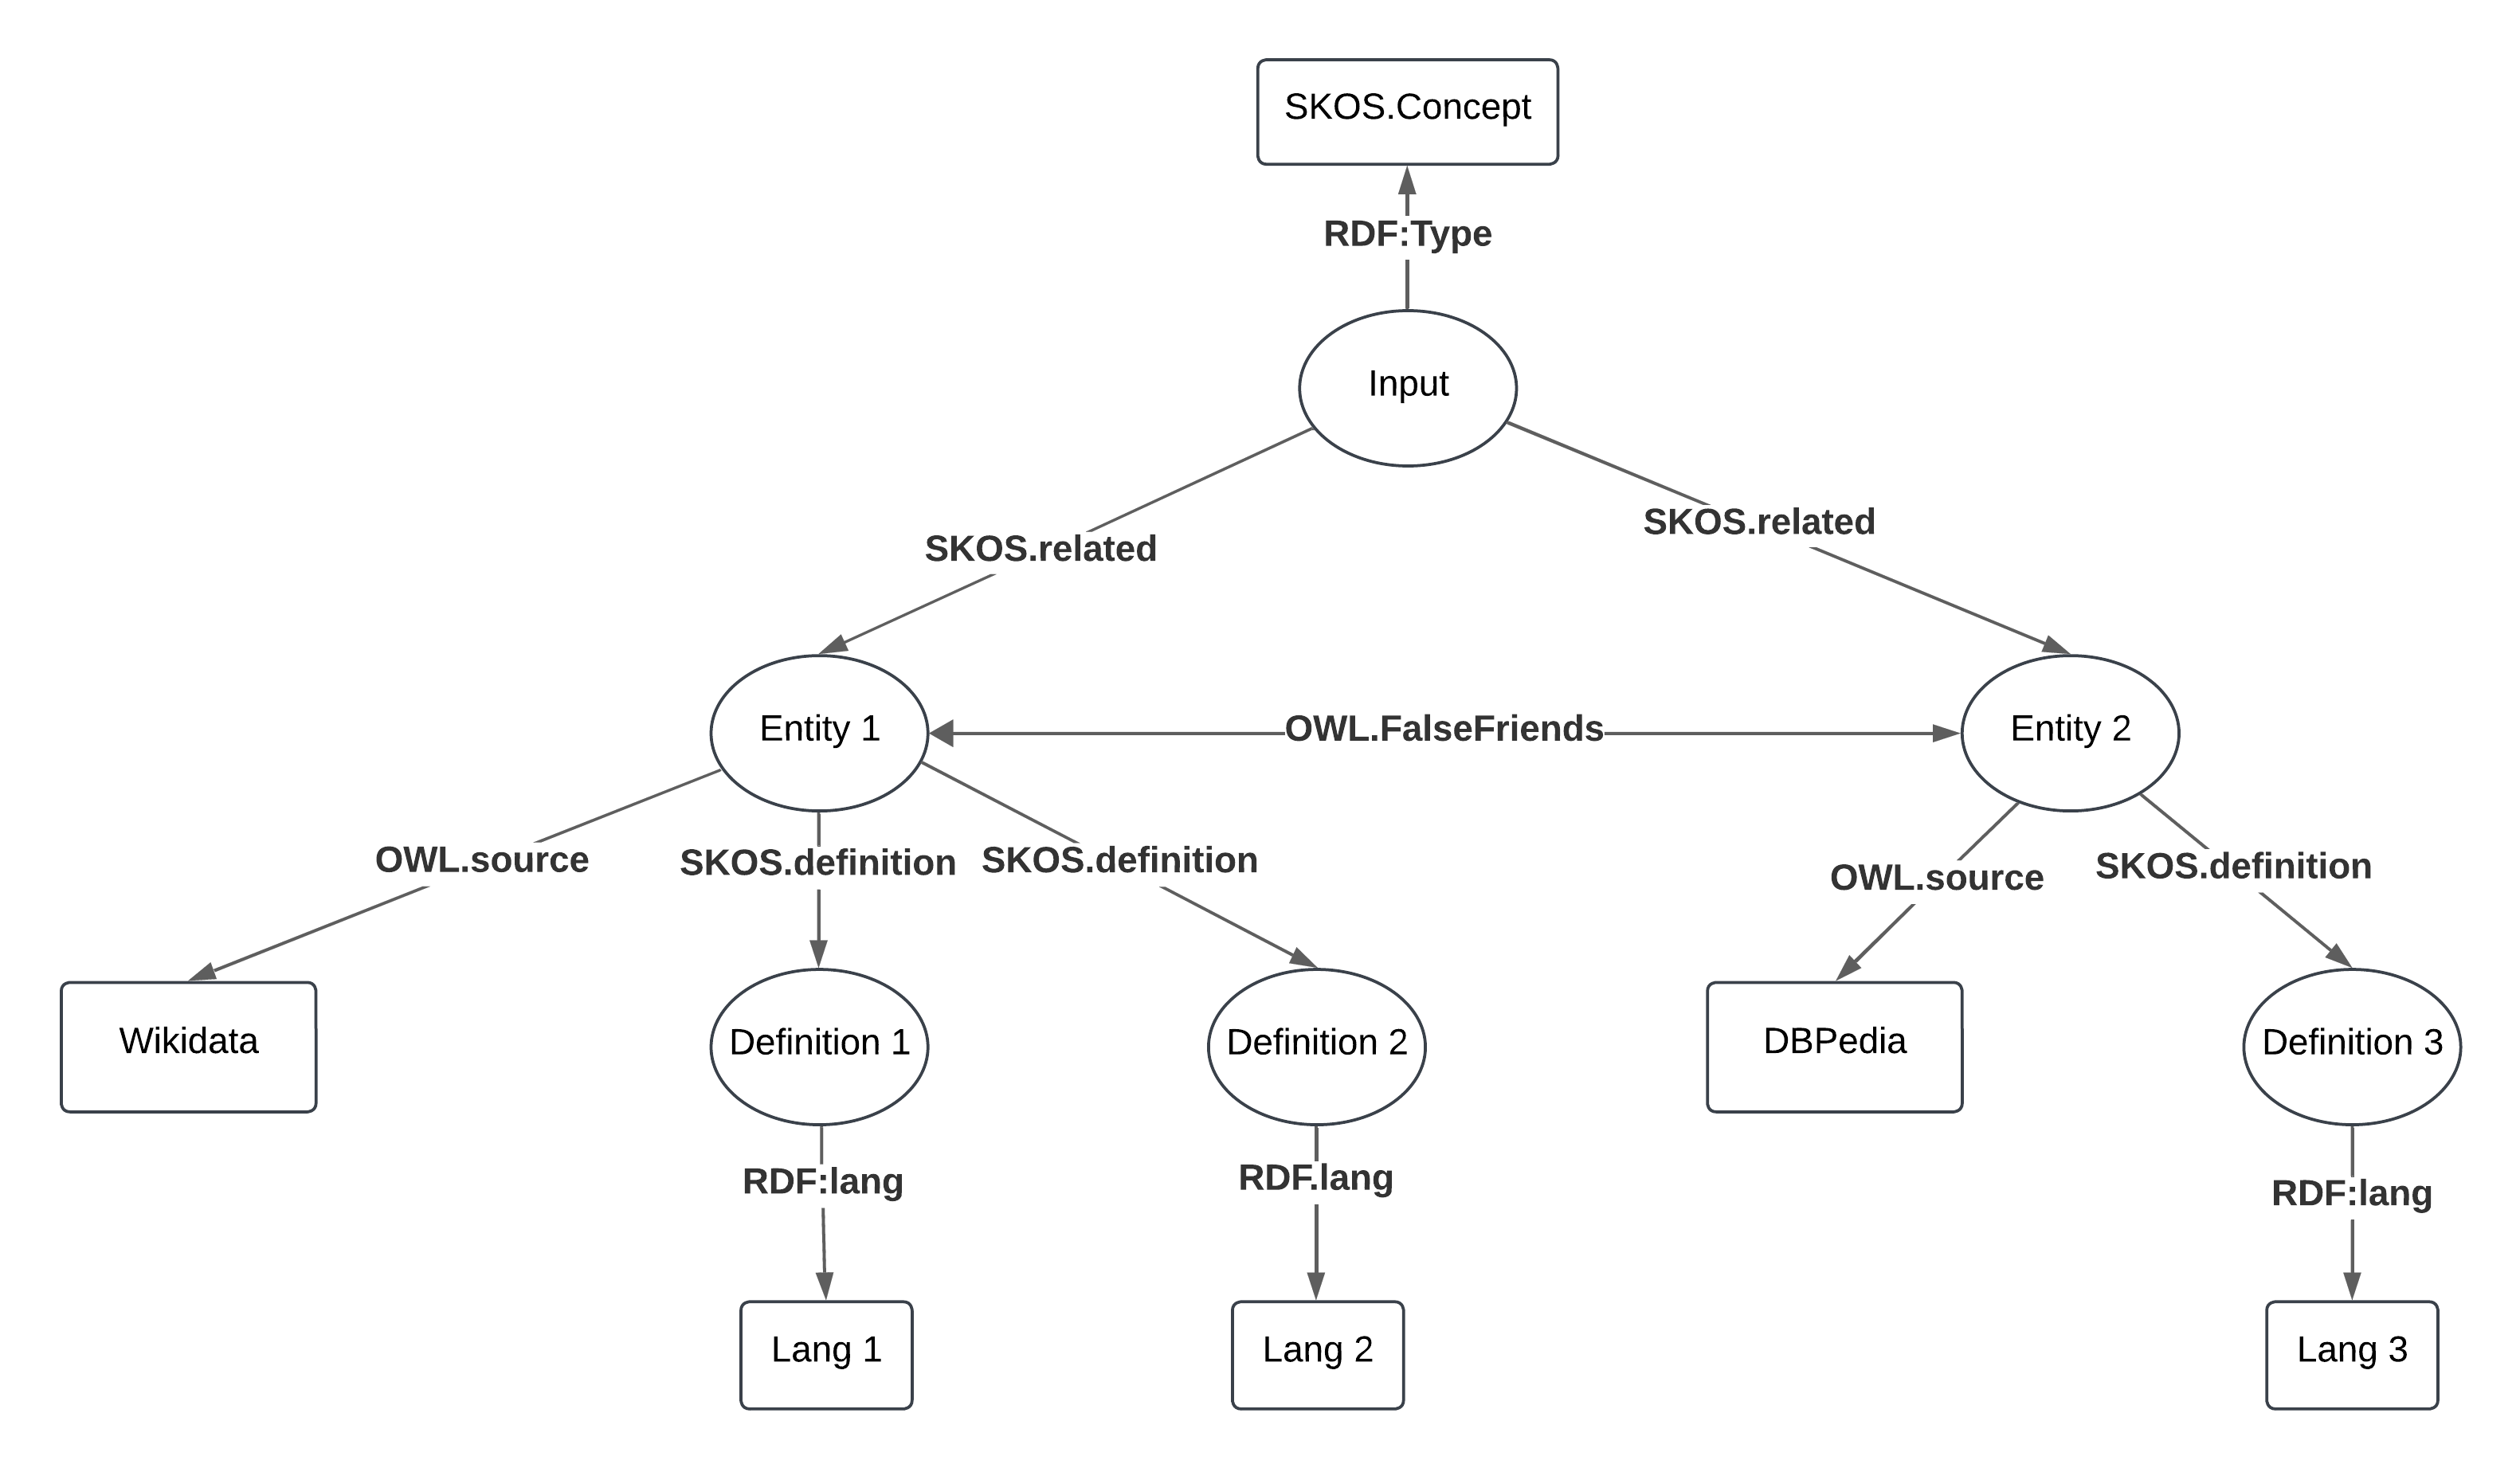
\includegraphics[width=0.80\textwidth]{Images/Grafos RDF.png}
    \caption{Wordify RDF resultant graph structure}
    \label{fig:graph}
  \end{center}
\end{figure*}

\begin{figure*}
  \begin{center}
    \leavevmode
    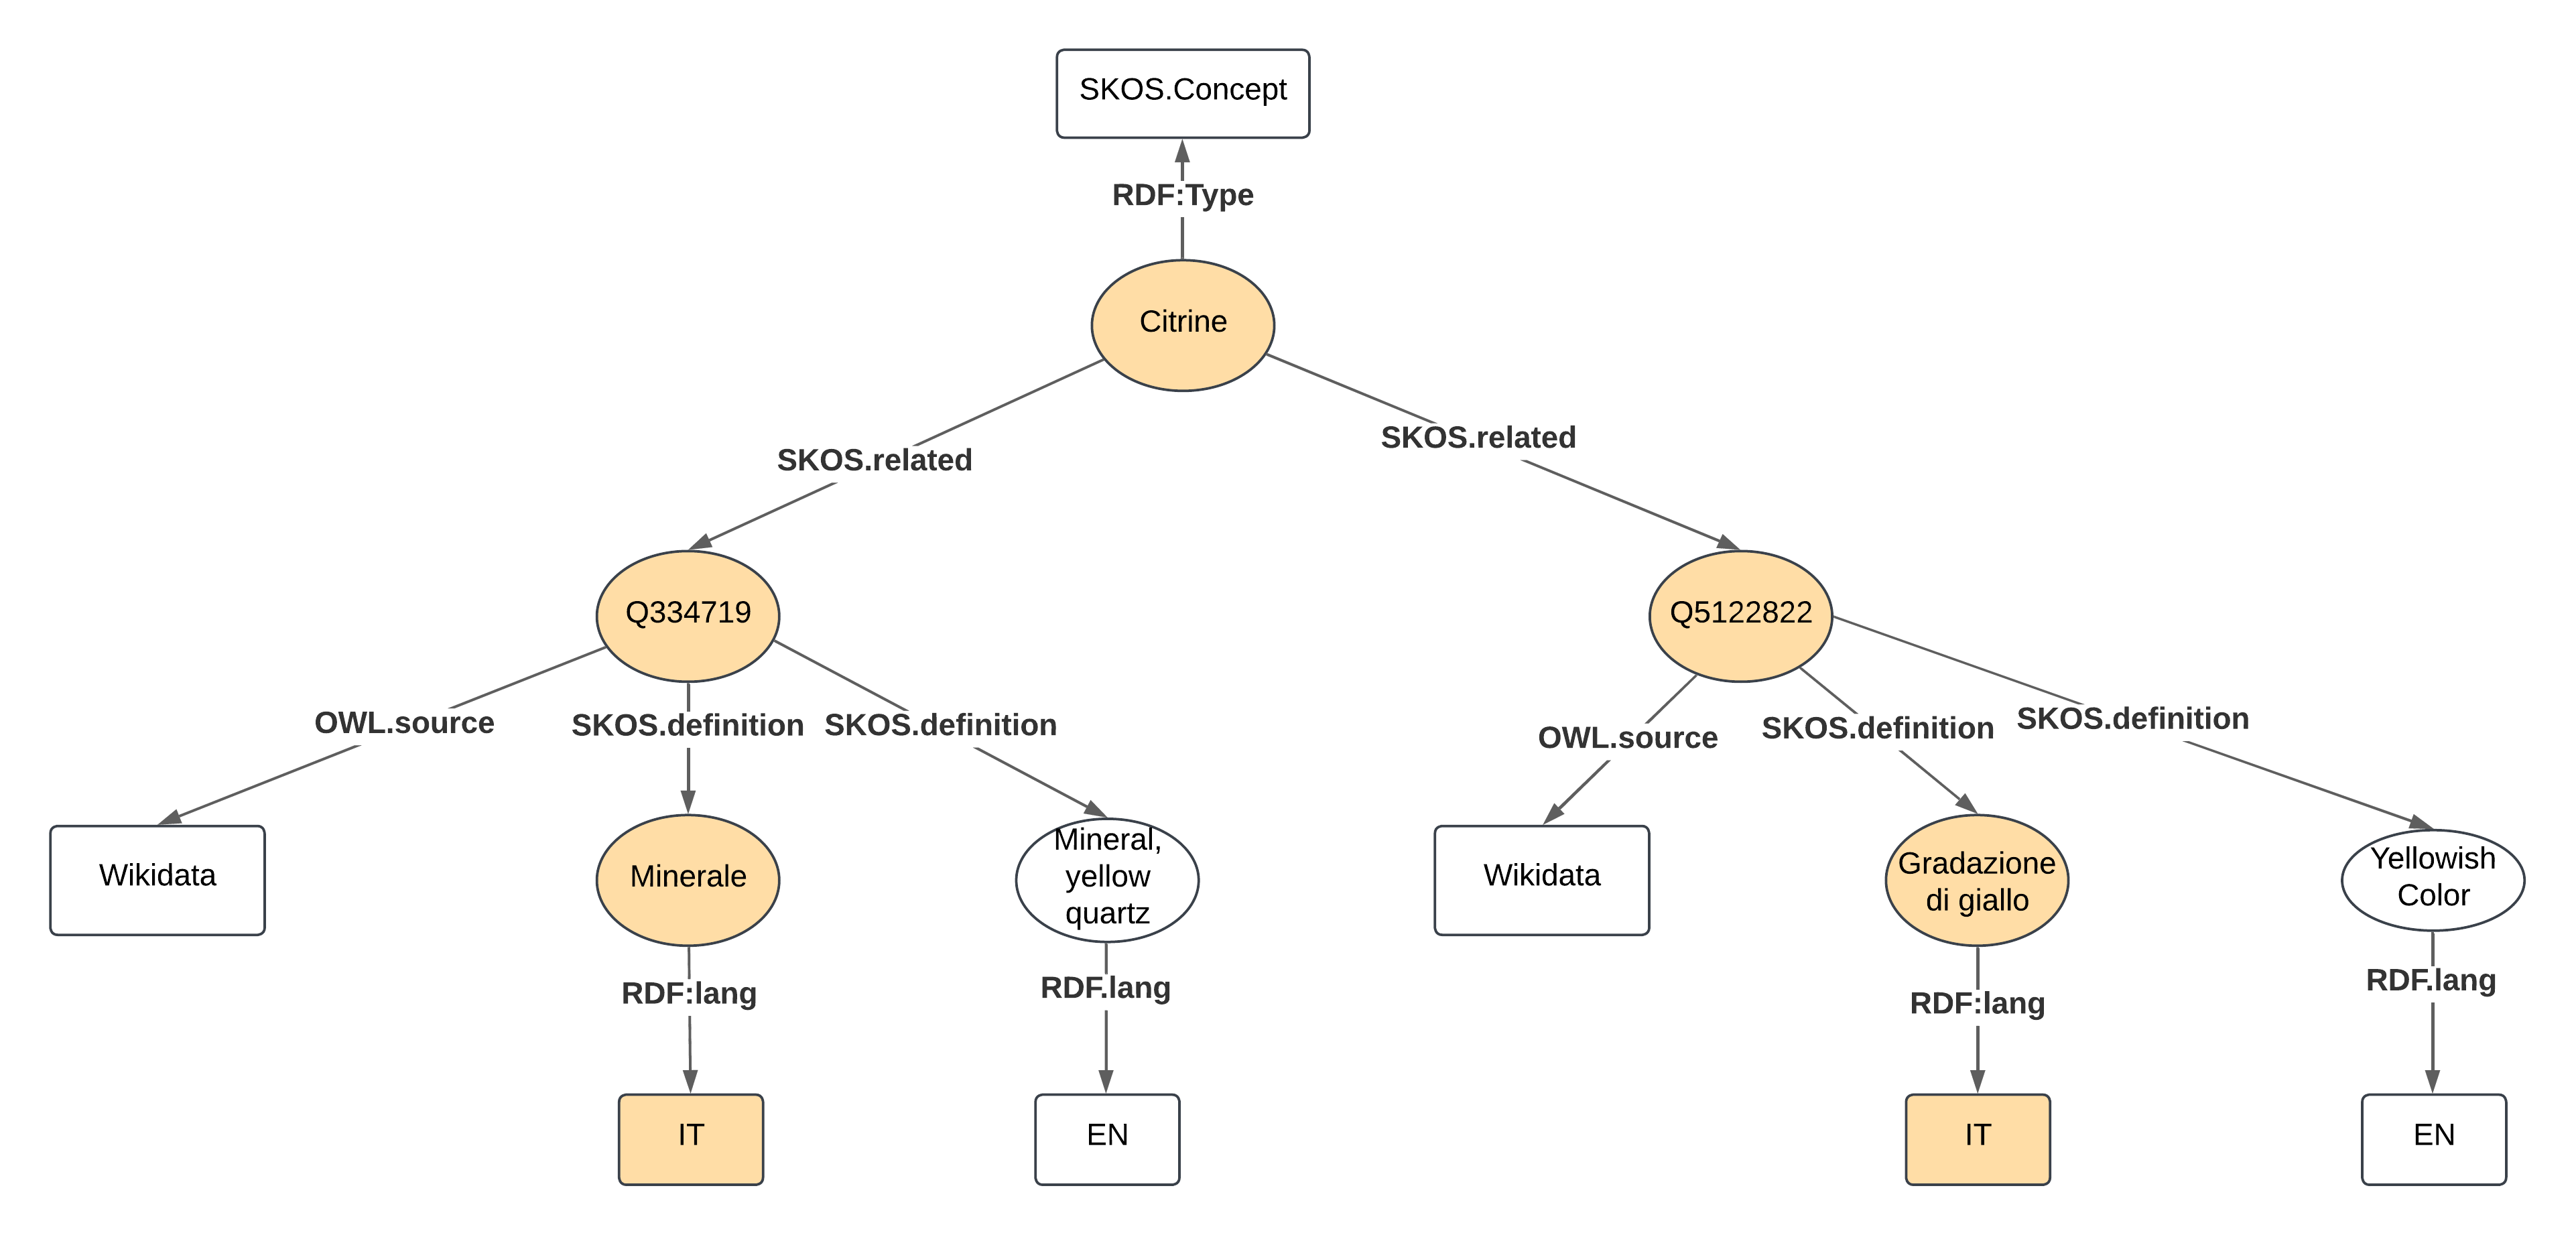
\includegraphics[width=0.80\textwidth]{Images/Grafos RDF - Ambiguidades.png}
    \caption{Computing ambiguities using Wordify graph}
    \label{fig:graph-ambiguities}
  \end{center}
\end{figure*}

\begin{figure*}
  \begin{center}
    \leavevmode
    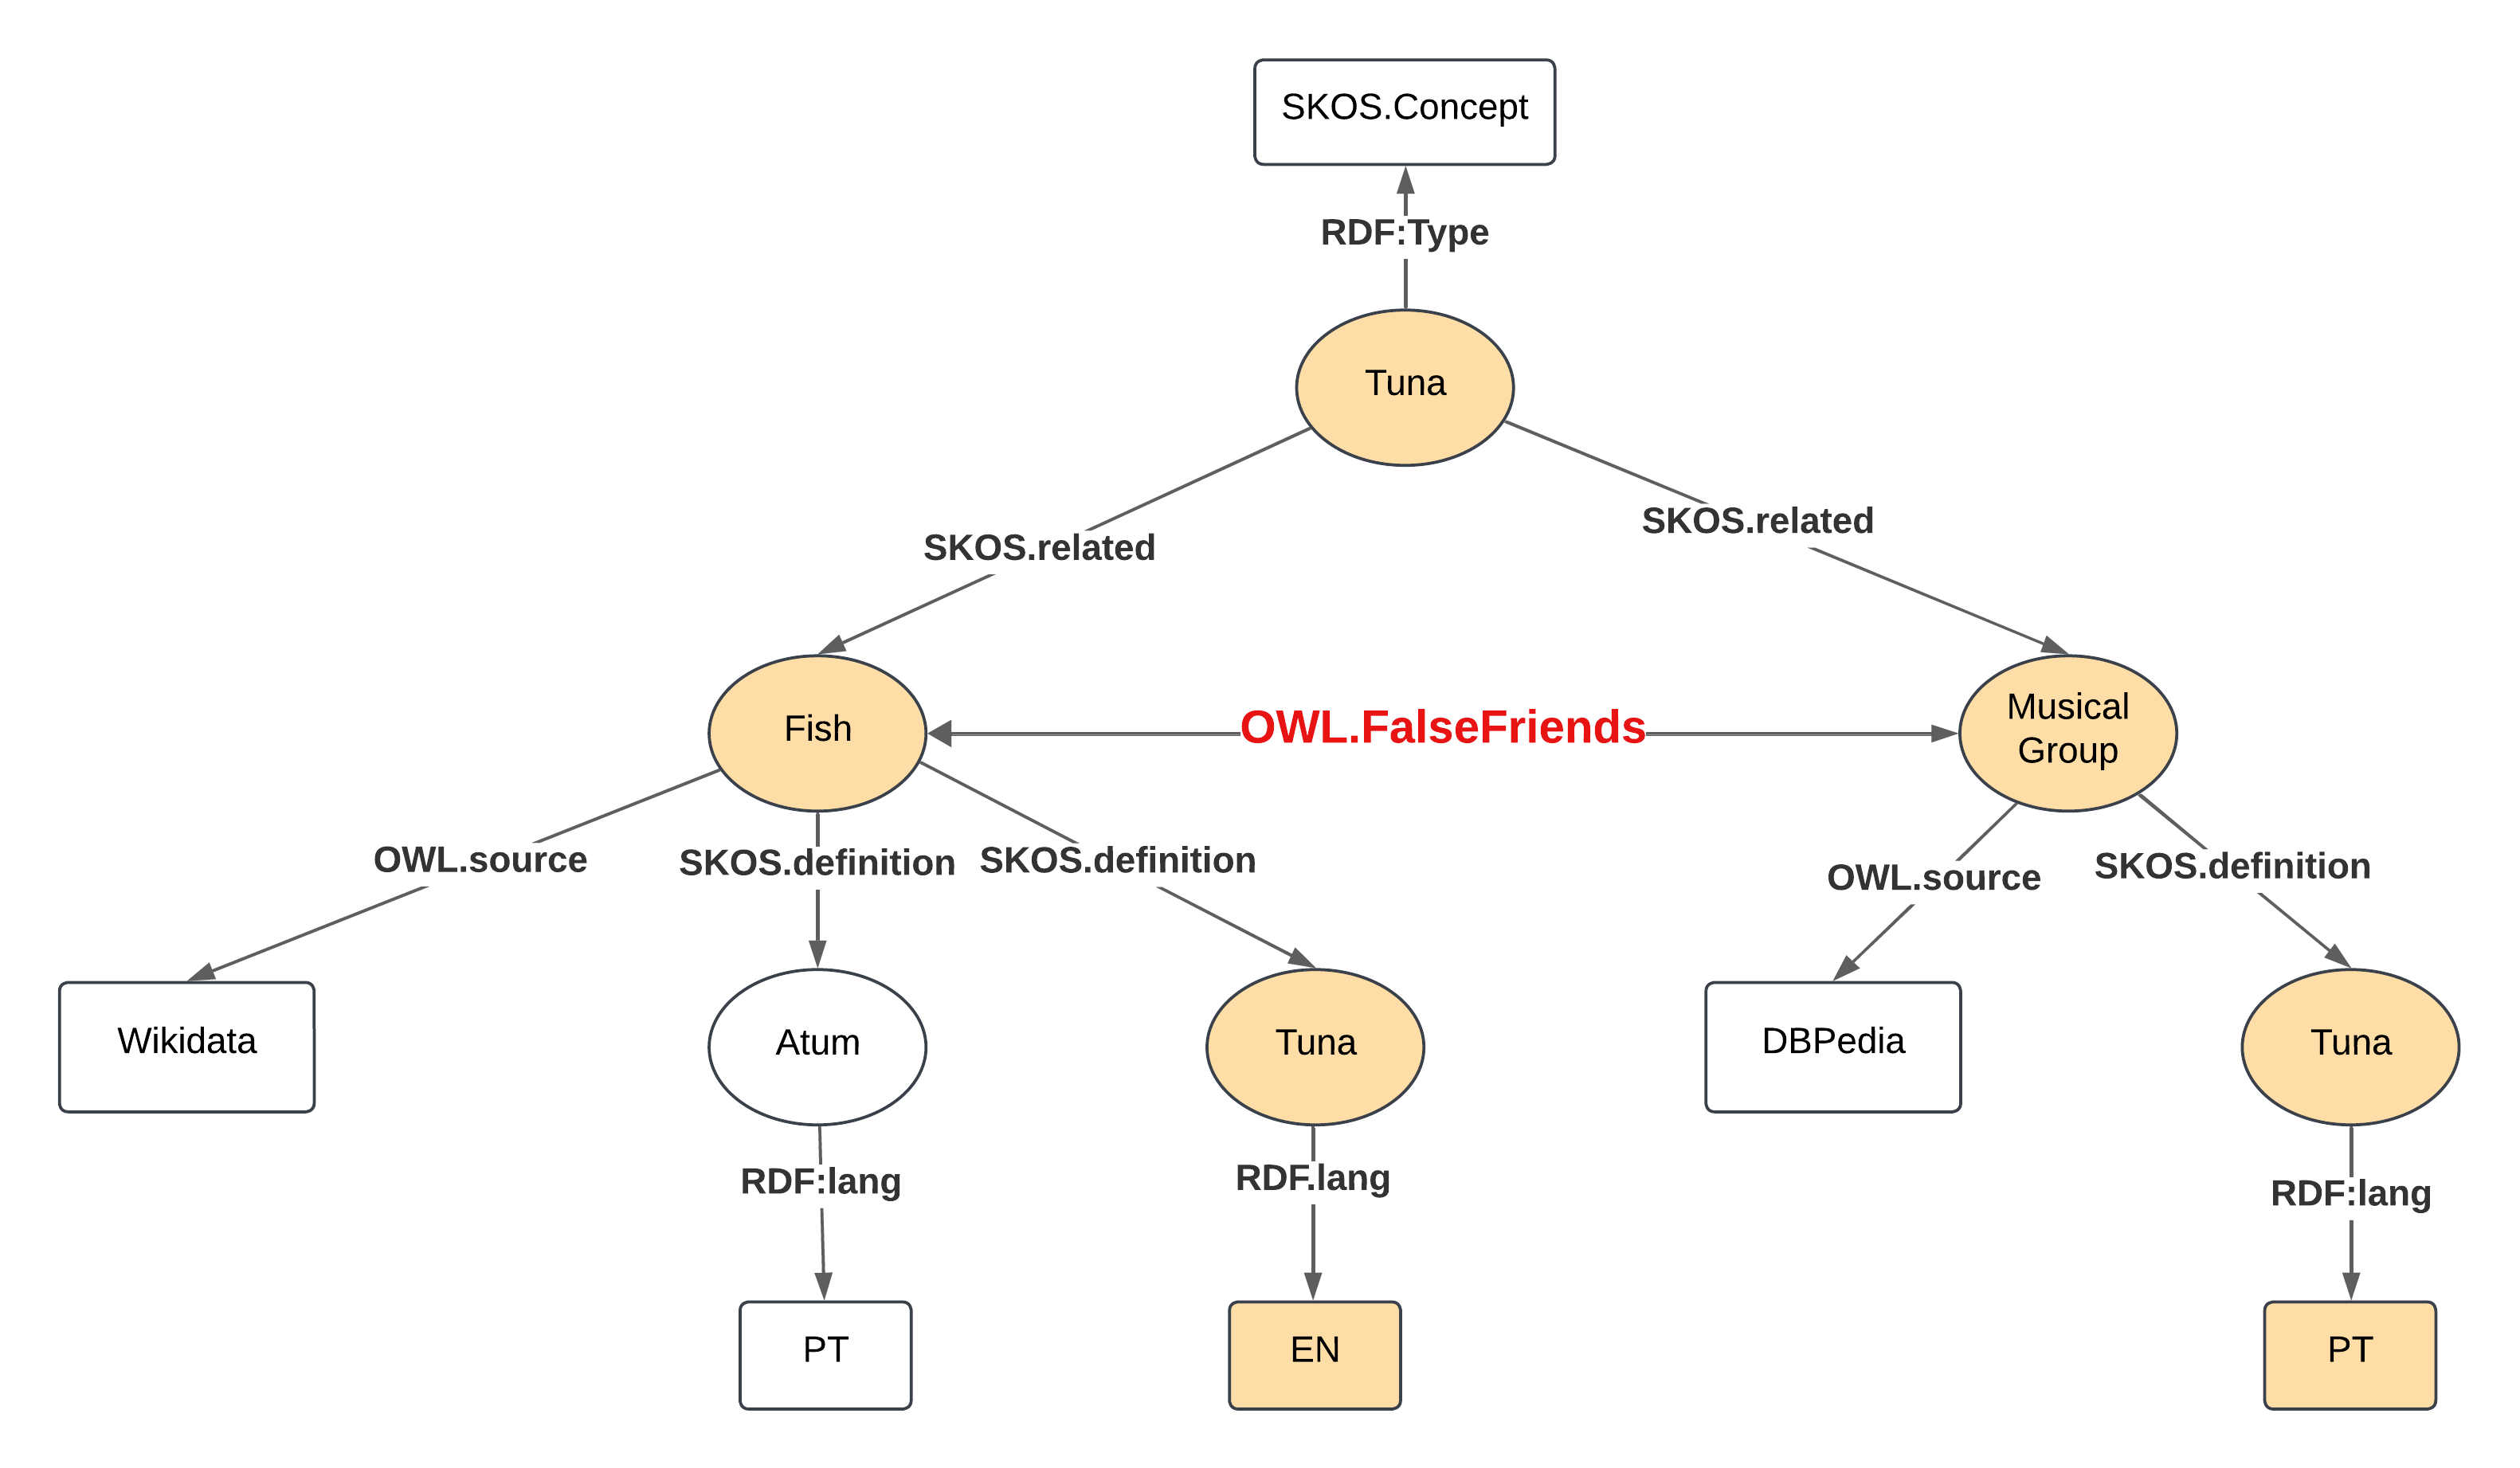
\includegraphics[width=0.80\textwidth]{Images/Grafos RDF - False Friends.png}
    \caption{Computing false friends using Wordify graph}
    \label{fig:graph-ff}
  \end{center}
\end{figure*}

\begin{figure*}
  \begin{center}
    \leavevmode
    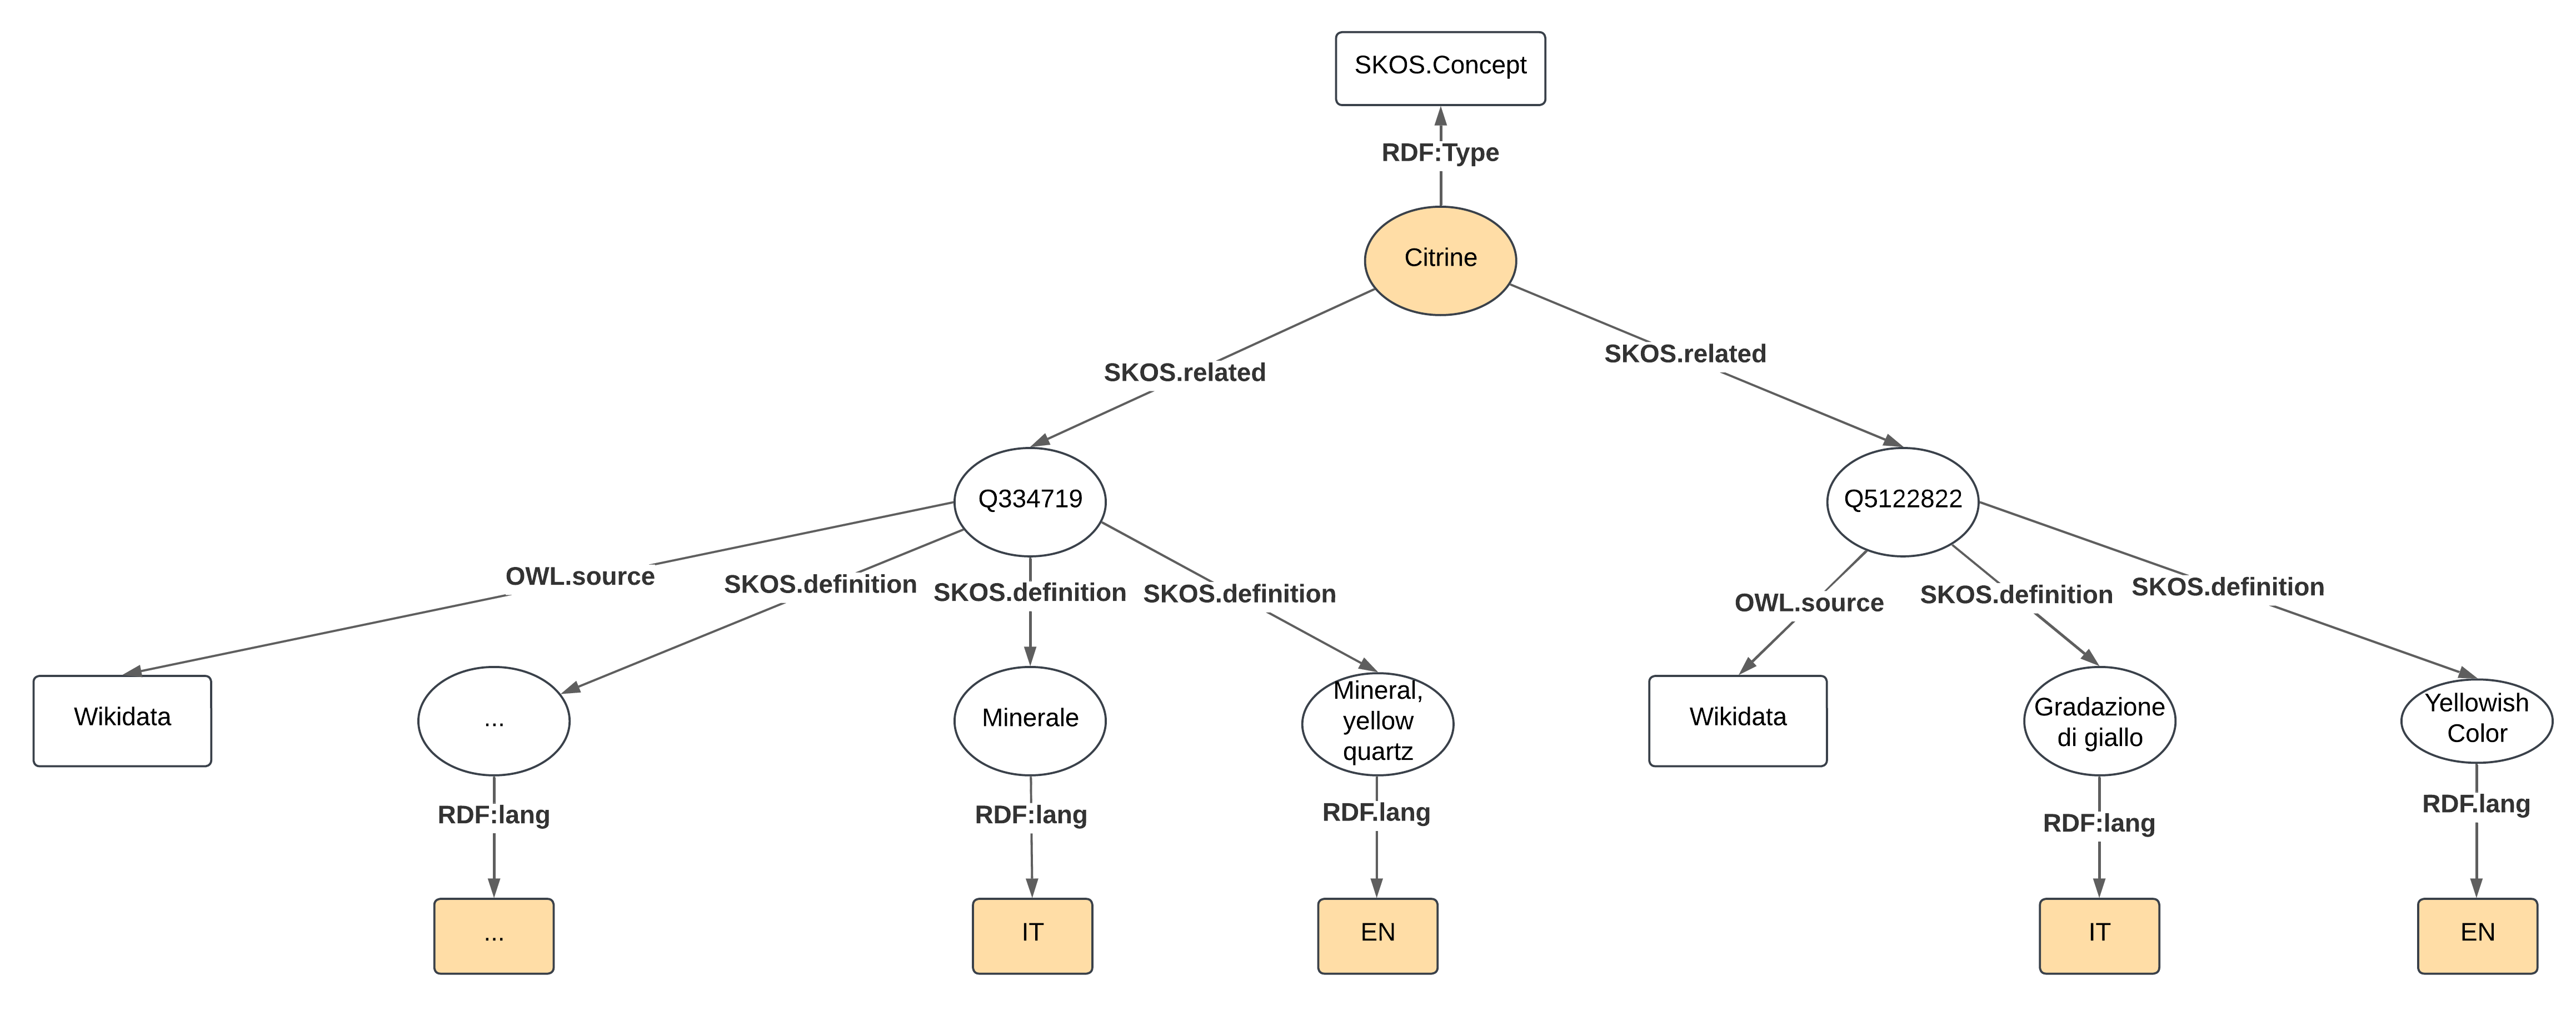
\includegraphics[width=0.80\textwidth]{Images/Grafos RDF - Languages.png}
    \caption{Computing languages using Wordify graph}
    \label{fig:graph-languages}
  \end{center}
\end{figure*}

\begin{figure*}
  \begin{center}
    \leavevmode
    \includegraphics[width=0.64\textwidth]{Images/limitedLanguages.png}
    \caption{The limited languages available for selection. The set of the languages were based on the most common languages in Europe, plus mandarin.}
    \label{fig:limitedLanguages}
  \end{center}
\end{figure*}

\begin{figure*}
  \begin{center}
    \leavevmode
    \includegraphics[width=0.64\textwidth]{Images/CrossDataLimitation.png}
    \caption{``Crow'' example, exposing the incapability to cross data between the knowledge bases, as they show different results for the same entity.}
    \label{fig:crossDataLimitation}
  \end{center}
\end{figure*}

\begin{figure*}
  \begin{center}
    \leavevmode
    \includegraphics[width=0.64\textwidth]{Images/imperialVSFine.png}
    \caption{The ``imperial'' and ``fino'' example, exposing Wordify's incapacity to identify regionalisms.}
    \label{fig:imperialVSFine}
  \end{center}
\end{figure*}

\begin{figure*}
  \begin{center}
    \leavevmode
    \includegraphics[width=0.64\textwidth]{Images/BeaksOfTheDuck.png}
    \caption{The ``bico de pato'' example, which shows that the system can only process single words.}
    \label{fig:Beaks}
  \end{center}
\end{figure*}

%----------------------------------------------------------------------------------------

\end{document}